\documentclass[11pt,a4paper]{article}
\usepackage{anysize}
\paperwidth=21cm \paperheight29.7cm
\marginsize{1.5cm}{1.5cm}{1.5cm}{1.5cm}
\usepackage[utf8]{inputenc}
\usepackage[magyar]{babel}
\usepackage[T1]{fontenc}
\usepackage{amsmath}
\usepackage{amsfonts}
\usepackage{amssymb}
\usepackage{graphicx}
\begin{document}
\noindent
\section{Ismertesse a mikroprocesszor alapú irányító berendezések csoportosítását, és alkalmazási területeiket! Ismertesse a Programozható Logikai Vezérlők definícióját és kiviteli formáit!}
	\subsection{A mikroprocesszor alapú irányító berendezések}
Hagyományosan az irányító berendezéseket segédenergiájuk alapján is  csoportosítják. Ennek megfelelően vannak mechanikus, pneumatikus, és villamos irányító rendszerek. A villamos irányító berendezéseket elektromechanikus (relés), huzalozott elektronikájú, és mikroprocesszor alapú (programozható) típusokra osztják fel. Napjainkban, ahol csak lehet, programozható irányító berendezéseket alkalmaznak.
\begin{figure}[hbtp]
    	 \centering
		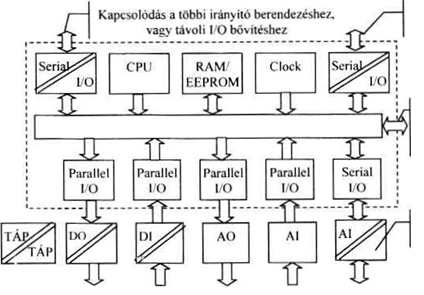
\includegraphics[scale=1.0]{1_mikroproc_blokk.png}
		\caption{A mikroprocesszor alapú berendezések blokkvázlata}
\end{figure}
A mikroprocesszor alapú irányító berendezések áramköri blokkvázlatát mutatja az 1. ábra. Az 1. ábrán a szaggatott vonallal körülhatárolt rész a közismert, bármely mikroprocesszort tartalmazó eszközre jellemző párhuzamos  buszos kialakítás.
Az illesztő áramkörök feladata az ipari jelszintekhez történő illesztés, és  a kielégítő zavarvédettség. A párhuzamos ferde egyenesek az illesztő áramköri blokkban jelzik a galvanikus leválasztást. A galvanikus leválasztás miatt szükséges az illesztő áramkörök, és a szaggatott vonallal körülhatárolt belső áramkörök független tápellátása.
\subsubsection{Mikrokontrollerek}
A mikrokontroller (mikroszámítógép) az alap áramköri elemek (CPU. RAM, SIO, stb.) NYÁK lapon kialakított kombinációja. Nincs ipari körülmények közötti működésre felkészítve. A programozása: CPU assembler. vagy magas szintű programozási nyelv (QBasic, QuickC) felületet biztosító. külön termékként megvehető, fejlesztő rendszer. Az illesztő áramkörök és a tokozás megtervezése is a termékfejlesztés része.
Alkalmazási területe: Nagy, közepesen nagy sorozatban gyártott termékekben, csak az adott feladatra kifejlesztett és optimalizált vezérlő berendezése. (háztartási gépek, autó elektronika, stb.)
Az ipari körülmények elviselését igazoló tesztelési eljárások költsége miatt gazdaságtalan az. egyedi vagy kis sorozatú alkalmazása. mert minden konkrét gépcsoport irányítása — még a nagyon hasonló feladatok is - egyedi alkalmazás. A kivitelezőnek a hatóságok felé igazolni kell a hardver ipari körülmények közötti alkalmazhatóságát, és a megbízható rendszerszoftvert. Az ipari kivitelű ($PLC$, Folyamatirányító, stb.) eszközökben ezt a gyártó garantálja,
Megjegyzés: A kis sorozatot vagy egyedi berendezést gyártók részére a beágyazott (embedded) ipari kivitelű számítógép alaplapokat ajánlják. Az ipari kivitelű számítógép alaplap ipari tokozásban, szabványos műszervázba (rack) helyezhető kivitelben, és ipari csatlakozókkal felszerelve kerül forgalomba.

	\subsubsection{Személyi számítógép alapú rendszerek}
	Hardveresen személyi számítógép alaplapú eszközök. Két árban nagyon eltérő csoportjuk van. az olcsóbb félipari, és a drága ipari kivitelű.
A félipari kivitelű PC alkalmazási területe: Elektromágneses zajterhelés szempontjából tiszta, közepesen nagy. és kis technológiák (irodaépületek, gyártásközi ellenőrzés. stb.); berendezések komplett irányítása. mérési adatgyűjtés (környezet monitorozás, térfigyelés, stb.); mérésanalízis (tesztlabor). A félipari kivitelű PC rendszerprogramja Windows CE, vagy Linux. Az alkalmazás programozására gyártó specifikus programnyelveket fejlesztettek ki.
Az ipari PC elektronikus zajjal terhelt, poros, párás környezetben való működésre felkészített berendezés. Az ipari kivitelű PC alkalmazási területe: Ipari környezetben működő, nagy számítási berendezések (több tengelyes hegesztő robotok, stb.); nagy adatkezelés igényii feladatok (automatizált raktárbázis. stb.) irányítása. Az ipari kivitelű PC-ben az alaplap és tokozása. a képernyő, a billentyűzet mind-mind ipari kivitelű és védettségű. A rendszerprogramja a gyártó által fejlesztett, 
	\subsubsection{Folyamatirányítók}
	Nagy és/vagy nagyon megbízható működést igénylő energetikai vagy vegyipari jellegű technológiák irányítására felkészített, hardveresen kész, szabványos irányítástechnikai programnyelveken programozható berendezések. Felkészített a redundáns működésre. Ez azt jelenti, hogy duplikálva vannak a modulok ($CPU$, hálózat, $I/O$). Az éppen működő az elsődleges (primer), míg a másik a tartalék (secondary). Ha az elsődleges meghibásodik, a tartalék veszi át (nagyon gyorsan) a szerepét.
	\begin{figure}[hbtp]
    	 \centering
		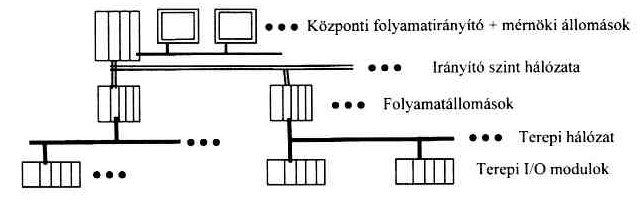
\includegraphics[scale=0.7]{2_folyamati_blokk.png}
		\caption{Folyamatirányító rendszer felépítése}
\end{figure}
A 2. ábrán létható folyamatirányító rendszer több különböző típusú irányító és terepi szintű hálózatot, valamint több ezer folyamatváltozót ($I/O$) képes kezelni. A központi folyamatirányító és a folyamatállomások egyenrangú intelligens eszközök.
Mindegyik futtatja a saját irányító szoftverét.
A folyamatállomások irányító szoftverei és a megjelenítő/mérési adatgyűjtő ($SCADA$) szoftver közös adatbázisból dolgozik, ami azért előnyös, mert bármelyik intelligens gép láthatja bármelyik változót a sok ezerből, és ezeket a  változókat csak egyszer kell definiálni. 
A folyamatállomások irányító szoftverei jól felkészítettek szabályozási feladatokra. Számos szabályozási algoritmust tartalmaznak. 
\subsubsection{Nem általános célú irányító berendezések}
Ezek a feladatok megvalósíthatók $PLC$-vel is, de kétféle megfontolásból külön gyártmánycsaládok alakultak ki.
\begin{enumerate}
	\item[•]Jól tipizálható feladatokat hajtanak végre, így speciálisan a feladathoz illesztett hardver és szoftver modulokból épül fel a rendszer. Ezért költséghatékony az új alkalmazás tervezése, kivitelezése. Idetartoznak az Épületautomatizálási és az Épület felügyeleti irányító rendszerek.
	\item[•] 	Az alkalmazott hardver és szoftver elemekre hatósági előírások vonatkoznak. A minősítési eljárás időigényes és költséges. A gyártók garantálják, hogy a hardver és szoftver moduljaik megfelelnek a hatósági előírásoknak, így az engedélyezési eljárás gyors. Idetartoznak a Tűzjelző, és a Kazánvezérlő irányító berendezések, rendszerek.
\end{enumerate}
\subsection{Programozható Logikai Vezérlők ($PLC$)}
A $PLC$-k (Programmable Logic Controller) ipari körülmények közötti működésre felkészített, hardveresen kész (illesztő áramkörök, táp, tokozás), szabványos irányítástechnikai programnyelveken ($IEC61131-3$) programozható berendezések. A speciális rendszerszoftver a berendezések része.
A $PLC$-k alkalmazási területe: Nagy, közepesen nagy, kis technológiák berendezéseinek, valamint egyedi gépek komplett irányítása, elsődlegesen vezérlése. Jelenleg ezek a legelterjedtebb ipari irányító berendezések. A gyártók a piaci igényekhez igazodva a $1O — 12 I/O$-t igénylő egyszerű logikai összefüggéseket tartalmazó feladatoktól, a több ezer $I/0$-t kezelő bonyolult szabályozásokat is tartalmazó feladatokig kínálnak kész hardvereket.
\subsubsection{Kompakt kialakítású $PLC$-k}
Egyetlen zárt tokban — kompakt, azaz tömbös felépítésben - elhelyezkedő, kötött számú ($1O$ — $30$) be, és kimenettel, és korlátozott szoftver erőforrással rendelkező eszközök. Általában nem, vagy csak korlátozottan bővíthetők. Tipikus alkalmazási területük az egyedi gépek vezérlése. A CPU képességeitől függően $50$ — $150$ eFt között van az áruk.
Napjainkban a Vezérlő relék (Control Relay) kezdik kiszorítani a piacról a kompakt $PLC$-ket. A vezérlő relék hardver kialakítása hasonlít a kompakt $PLC$-k hardver kialakításához. A vezérlő relék abban különböznek a kompakt $PLC$-éktől, hogy nem a szabványos ($IEC61131-3$) programozási nyelveken, hanem gyártó specifikus, kisszámú grafikus szimbólumot tartalmazó, leegyszerűsített programozási nyelveken programozhatók, és programfutás közben (online) nem írható át a programjuk, vagyis minden programmódosításkor le kell állítani az irányított berendezést.
\subsubsection{Modulárisan kompakt kialakítású $PLC$-k}
A 3. ábra ilyen $PLC$-k elrendezését ábrázolja. Szokványos szerelő sínre pattinthatók. A lokális $I/O$ bővítések belső buszát rövid szalagkábellel kötik  össze. A többi $I/O$ modul soros adatátviteli hálózaton keresztül érhető el.
\begin{figure}[hbtp]
    	 \centering
		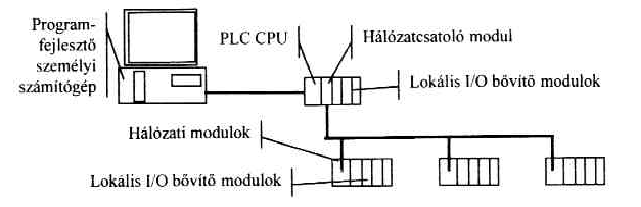
\includegraphics[scale=0.7]{3_modularis_plc.png}
		\caption{Moduláris $PLC$-k struktúrája}
\end{figure}
\begin{enumerate}
	\item[•]Különböző sebességű $PLC$ $CPU$-k, különböző méretű memóriával válaszható. Szoftveres képességekben (pl.: lebegőpontos számításra képes, vagy sem) is lehet különbség az egyes $CPU$ típusok között.
	\item[•]Különböző hálózati modulok (CANOpen, Profibus DP, Interbus S, stb.) választhatók.
	\item[•]A kiválasztott $CPU$-hoz, valamint a hálózati modulokhoz lokálisan különböző típusú (pl.: 16 diszkrét bemenet, vagy kimenet, 8 — 8 diszkrét be-, kimenet, vagy 8 analóg bemenet, 4 analóg kimenet, 4 — 2 analóg be, kimenet, stb.) $I/O$ modulok fűzhetők. Így az adott alkalmazáshoz legjobban illeszkedő be, kimenetszám állítható össze. A tipikus maximális terjedelem 800 be, vagy kimeneti jel.
	\item[•]A hálózatra különböző intelligens eszközök (frekvenciaváltó, MMI, stb.) fűzhetők fel.
\end{enumerate}
Tipikus alkalmazási területük a közepes technológiák, gépcsoportok vezérlése. A $CPU$ képességeitől és a modulok típusától függően 200 — 500 eFt  között van az ára egy 50 $I/O$-t tartalmazó kiépítésnek
\subsubsection{Modulvázas (rack) kialakítású $PLC$-k}
A nagy teljesítményű, nagy sebességű $PLC$ $CPU$-k kedvelt kiviteli formája. Szerelősín helyett modultartó vázba (rack) kerülnek a zárt tokban elhelyezkedő modulok. A modultartó váz hátlapjára szerelt NYÁK-on helyezkedik el a busz rendszer. A modulvázban 32 bites lokális $I/O$ modulok helyezhetők. Jellegzetes, de nem kötelező kialakítás, hogy modulvázban csak a nagy teljesítményű $CPU$, és a hálózati csatoló modulok vannak.
\begin{figure}[hbtp]
    	 \centering
		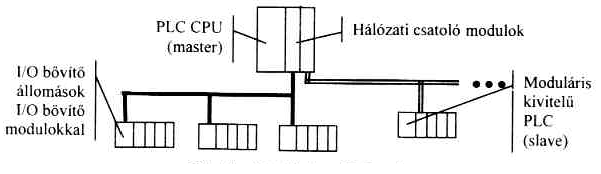
\includegraphics[scale=0.7]{4_rack_plc.png}
		\caption{Modulvázas $PLC$-k struktúrája}
\end{figure}
A hálózati csatoló modulokra $I/O$ bővítések, vagy egy-egy irányítási részfeladatot önállóan (saját vezérlő program) ellátó modulárisan kompakt PLC-k vannak felfűzve. Manapság elterjedten alkalmazott hálózat típusok: Profibus-DP. DeviceNet, CANopen, Modbus, Interbus-S).
A technológia vagy gépcsoportok működésének összehangolását a központi (master) modulvázas $PLC$ végzi. ha van is más intelligens eszköz a rendszerben, az alárendelt (Slave) üzemmódban dolgozik.
Tipikus alkalmazási területük a nagy vagy gyors technológiák, gépcsoportok vezérlése. Egy 500 - 800 $I/O$-t tartalmazó kiépítésnek a CPU képességeitől és a modulok típusától függően 6 — 10 mFt között van az ára.

\section{Ismertesse a $PLC$ felhasználói program struktúráját! Definiálja a funkció blokk és a függvény közötti eltérést! Ismertesse a ciklikus programfuttatás ütemeit, és a reakció idő összetevőit! }
\subsection{Programozható logikai vezérlők szoftverszerkezete}
A személyi számítógép rendszerszoftvere napjainkban tipikusan a Windows. A fejlesztő szoftver a program fejlesztő személyi számítógépen fut. A fejlesztő szoftverrel történik a felhasználói program megírása, szintaktikai ellenőrzése, lefordítása gépi kóddá, letöltése a $PLC$ $CPU$-ba. A fejlesztő szoftverrel lehet ellenőrizni a felhasználói program futtatását, online módon adatot módosítani, stb. A $PLC$ $CPU$-ban fut a gépi kódban letöltött felhasználói program. A felhasználói program írja le az adott konkrét alkalmazáshoz illeszkedő irányító algoritmusokat. A $PLC$ $CPU$-ban csak egyetlen alkalmazáshoz (technológiához) tartozó felhasználói program fut. 
A $PLC$-ben szintén fut egy rendszer szoftver, ami gyártó specifikus és a $PLC$ szerves része, nem cserélhető, nem módosítható. Ez futtatja a gépi kódban letöltött felhasználói programot, végzi az öntesztet, kezeli a megszakításokat, tartja a kapcsolatot a kezelővel.
\begin{figure}[hbtp]
    	 \centering
		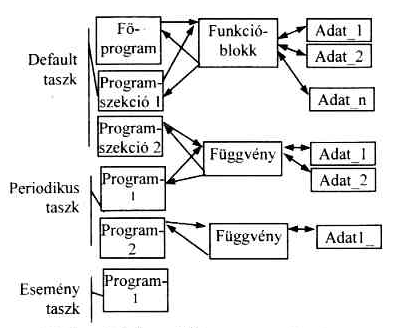
\includegraphics[scale=0.7]{5_plc_program_szerk.png}
		\caption{A felhasználói program szerkezete}
\end{figure}
Az 5. ábra mutatja a  felhasználói program szerkezetét. A felhasználói program, ha  az áttekinthetőség és a $CPU$ erőforrásának hatékony kihasználása érdekében szükséges, akkor részekre van bontva. Ezek a programrészek különböző típusú és prioritású taszkokban futtathatók.
A taszk együtt kezelendő programköteget jelent. A prioritás fontossági sorrendet határoz meg.
\\A taszkok típusai:
\begin{enumerate}
	\item[•]Alap (Default): Az ehhez rendelt programrészek (szekciók) programfeldolgozása ciklikus. Ebben fut a főprogram. Főprogramot minden alkalmazásnak tartalmaznia kell.
	\item[•]Periodikus (Cyclic): Az ehhez rendelt programok adott időközönként (10[s], 1[s], 100 [ms], stb.) periodikusan futnak le.
	\item[•]Esemény (Event): Az ehhez rendelt programok valamilyen változó, vagy változók logikai kombinációjának fel-, vagy lefutó élére futnak le.
	\item[•]Rendszer (System): Ezek a gyártó által készített, hiba lekezelést végző, legnagyobb prioritású programok Az 5. ábra nem tartalmazza. 
\end{enumerate}
A vezérlő reléknek és a legtöbb kompakt $PLC$-nek csak "Alap" taszkja és a felhasználó elől rejtett "Rendszer" taszkjai vannak, továbbá az "Alap" taszkban csak egy program futhat. A legnagyobb teljesítményű modulvázas $PLC$-kben "Periodikus" és "Esemény" taszkokból többféle típus van, így ezekben az irányító berendezésekben tucatnyi taszk, illetve program futtatható.
A taszkoknak prioritása van. A "Alap" taszk prioritása a legkisebb. A  magasabb prioritású taszk megszakítja az alacsonyabb prioritású taszk programjainak feldolgozását (6. ábra), lefut, majd folytatható az alacsonyabb prioritású taszk programjainak feldolgozása. A megszakítások egymásba ágyazhatósága napjainkban már nincs korlátozva.
\begin{figure}[hbtp]
    	 \centering
		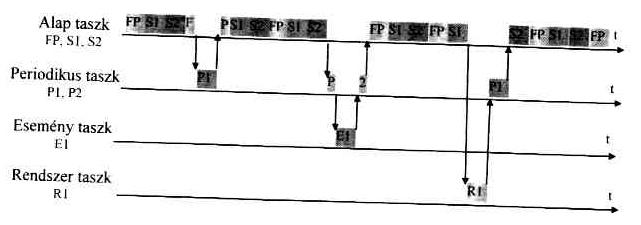
\includegraphics[scale=0.7]{6_tasz_futas.png}
		\caption{A taszkok és programjaik futtatása}
\end{figure}
A 6. ábra annyiból torzít, hogy a "Periodikus", az "Esemény", és a "Rendszer" taszk sokkal ritkábban használja a CPU időt. Az "Alap" taszkban  elhelyezett programok, amikor csak lehet, újra meg újra ciklikusan feldolgozásra kerülnek. A "Periodikus" taszk programjaihoz különböző periódus idő, az "Esemény" taszk programjaihoz különböző feltételek rendelhetők, ezért ezek programjai külön-külön kerülnek feldolgozásra. A "Rendszer" taszk hardver vagy szoftver hiba esetén kerül meghívásra- és a 6. ábrától eltérően legtöbbször megszakítja a felhasználói program feldolgozását.
Az 5. ábrán látható, hogy a programokból funkció blokkok és függvények hívhatók. Bármely funkció blokk és függvény többször, akár különböző programokból meghívható. A funkció blokk. és a függvény a gyakran előforduló (időzítések, számlálók, komparátorok, jeltípus konvertálók, aritmetikai műveletek, stb.) feladatok részére megírt szubrutinok.
\begin{enumerate}
	\item[•]A funkció blokk olyan szubrutin, amelynek több be-, és kimeneti változója lehet. A fordító program csak egyszer fordítja le a funkció blokkot, és  többszöri meghívás esetén csak a bemeneti (feldolgozandó adatok), illetve kimeneti (eredmények) változók részére foglal le programterületet. Ezek a memória területek bármely programból elérhetők.
	\item[•]A függvény olyan szubrutin, amelynek több be-, és csak egy kimeneti változója lehet. A kimeneti változó a $CPU$ munkaregiszterében képződik, ezért ha a következő programsor nem dolgozza fel, akkor elvész. A fordító program csak egyszer fordítja le a függvényt, és csak a bemeneti (feldolgozandó adatok) változók részére foglal le programterületet.
\end{enumerate}
A funkció blokkok és függvények lehetnek az $IEC61 131-3$ szabványban definiáltak (ezeket minden fejlesztőprogram kötelezően tartalmazza), a gyártó által felkínáltak, valamint írhat ilyent a felhasználó is (csak óvatosan, mert a gyártó által felkínáltak biztosan jól teszteltek).
A memóriaterületen és a $CPU$ sebességén túl, a $PLC$ típus megválasztásakor fontos szempont, hogy milyen típusú taszkokat képes kezelni, és hogy milyen funkció blokk és függvény könyvtárra van.
A vezérlő relékben a funkció blokk és függvény típusok száma csak egy  tucatnyi, és csak korlátozott alkalommal hívhatók. A legnagyobb teljesítményű   "Rack"-es $PLC$-kben a funkció blokk és függvény típusok száma 1000 körüli,  és korlátlan a meghívhatóságuk száma.
\begin{figure}[hbtp]
    	 \centering
		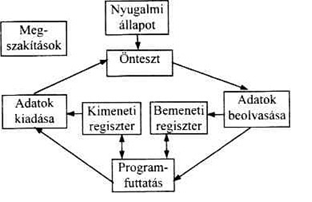
\includegraphics[scale=0.7]{7_ciklikus_plc.png}
		\caption{A ciklikus programfeldolgozás mód}
\end{figure}
A 7. ábrán a ciklikus programfeldolgozás ütemei láthatók.
\begin{enumerate}
	\item[•]Nyugalmi állapotban a felhasználói program gépi  kódba lefordítva a $PLC$-ben van, de nem fut.
	\item[•]Az önteszt a megszakításokkal nem lefedett (pl.: végtelen ciklus) hibákat kezeli.
	\item[•]Beolvasáskor az adatok, a fizikai bemenetekről a bemeneti regiszterbe kerülnek. 
 A továbbiakban a bemeneti regiszter adatait dolgozza fel a $CPU$, így elkerülhető a hazárd.
 Megjegyzés: A hazárd hiba abból keletkezne, hogy egy ciklusban egy bemeneti adat különböző értékkel kerülne feldolgozásra, mert programfeldolgozás közben változott meg a bemenet értéke.
	\item[•]A program futtatása az "Alap" taszk feldolgozását jelenti. A felhasználói program feldolgozásának egy ciklusa akkor fejeződik be, amikor az "Alap" taszk programjai mind feldolgozásra kerültek. 
	\item[•]Az adatok kiadásakor a programfeldolgozás közben a kimeneti regiszterbe került adatok a fizikai kimeneti áramkörökre kerülnek. Ezután újabb önteszttel elölről kezdődik a ciklus.
	\item[•]Megszakítást kezdeményeznek az "Esemény", a "Periodikus", és a "Rendszer" taszkok, valamint a kezelői beavatkozások.
\end{enumerate}
A sorrendi programfeldolgozás következtében a $PLC$ valamely bemenetén történt jelváltozás hatása nem azonnal jelenik meg a kimeneteken. Ez a késlekedés a reakcióidő. A reakció idő fontos a $PLC$ típus megválasztásakor, mert értelemszerűen kisebbnek kell lennie, mint a kiadott vezérlő parancs végrehajtásának ideje.\\\\
Reakció idő megbecsülhető az összetevőiből. Az összetevők:$$T_R = 2 * T_C + T_F + T_D + T_N + \sum_{}^{}T_I$$
\begin{enumerate}
	\item[•] $T_R$: A reakció idő, amely ahhoz szükséges, hogy a bemeneten történő jel változás hatására megváltozzon a kimenet
	\item[•] $T_C$: A ciklusidő, ami az önteszttől öntesztig szükséges időtartam. A programfeldolgozás a bemeneti regiszterből történik; de legrosszabb esetben sem kell két ciklusidőnél több a bemeneti jelváltozás feldolgozásához.
A $T_C$ ciklusidő függ a $CPU$ sebességétől és a felhasználói program hosszától, valamint hogy milyen típusú utasításokat tartalmaz a program. A katalógusok 1024 (l Kszó) átlagosan előforduló utasítássor lefutásához szükséges időt adják meg. A vezérlő relék ciklus ideje 5-10 ms, a moduláris $PLC$-k ciklus ideje 1-2 ms, modulvázas $PLC$-k ciklus ideje 0,5 ms, a különlegesen gyors $PLC$-k 0,1 ms, vagy még kisebb ciklusidővel rendelkeznek.
Megjegyzés: 1 Kszó program általában elegendő 30-40 $I/O$-val rendelkező berendezés irányítására.
	\item[•] $T_F$: A bemeneten levő $RC$ szűrő időállandója, amelynek tipikus értéke Európában 2 ms. (A hálózati 50 Hz periódus ideje 20 ms. Számos $PLC$-nél szoftveresen módosítható az analóg szűrés időállandója.
	\item[•] $T_D$: A tranzisztoros kétállapotú kimeneteken, az induktív terhelés ellentétes polaritású visszahatását mérsékelő, $RC$ csillapítótag idöállandója, vagy a  reed-relés kimeneteken a tekercs megszólalási idejc. Tipikus érték: 1 ms.
	\item[•] $T_N$: A hálózati állomások lekérdezési/frissítési ideje.
A modulárisan kompakt kialakítású $PLC$-k esetén a tipikus érték $I/O$  állomásonként 0,5-1 ,5 ms.
A modulvázas $PLC$-kben 4 hálózati csatoló modul, és modulonként 31 $I/O$ bővítő állomással az összes be-, és kimenet lekérdezési/frissítési ideje kisebb, mint 0,1 -0,5 ms. Ezt az alábbi szervezés teszi lehetővé.
A hálózati csatoló modulokban szintén van $CPU$, amelyek a $PLC$ $CPU$-val párhuzamosan dolgozva adatot cserél a hálózat $I/O$ bővítő állomásaival. Az adatcsere a saját be-, és kimeneti regiszter területei és a saját hálózatán levő $I/O$ bővítő modulok be-, és kimenetei között zajlik, és jellegzetesen rövidebb ideig tart, mint a $PLC$ $CPU$ ideje. A $PLC$ $CPU$ és a hálózati csatoló modul $CPU$ be-, és kimeneti regiszterei a 7. ábrán látható adatbeolvasás fázisban cserél adatot.
	\item[•] $\sum_{}^{}T_I$: A megszakítás programok feldolgozásának ideje az adott ciklusban. A legrosszabb, és meglehetősen valószínűtlen, ha valamennyi program feldolgozásra kerül az adott ciklusban.
\end{enumerate}
\section{Jellemezze a távadók és a végrehajtók generációi! Mit jelent a 2, 3, 4 vezetékes bekötés? Adja meg a leggyakrabban alkalmazott szabványos ipari jeltartományokat!}
A villamos távadókat kimeneti jelük. a villamos végrehajtókat bemeneti jelük és működési módjuk szerint csoportosítják különböző generációkba:
\begin{enumerate}
	\item[•]"C" generációs: Analóg működésű. szabványos ($0/4-20mA$, $0/2-10V$) analóg áramjelű, vagy feszültségjelű távadók, végrehajtók.
	\item[•]"D" generációs: Digitális működésű, egyen analóg jelre ültetett frekvencia modulált analóg jelű (smart) távadók, végrehajtók. A szabványos egyen analóg jel egy-, a frekvencia modulált analóg jel kétirányú.
	\item[•]"E" generációs digitális távadók, végrehajtók. A digitális jelek terepi buszon közlekednek. A terepi buszon kétirányú a kapcsolat, az eszköz nem csak alapfeladatát látja el, hanem automatikusan vagy lekérdezésre az állapotáról is küld információt.
\end{enumerate}
A generációs eszközök az alkalmazott $4-20 mA$ szabványos áramjelet $\rm 0,5mA$ amplitúdójú és egy adott időablak hosszúságú, kétféle frekvenciájú (Bell 202 szabvány esetén például $2200 Hz = L, 1200 Hz = H$) szinusz jellel modulálja. A moduláló jel digitális jelet képez, amellyel kétirányú adatforgalom valósítható meg az irányító berendezés vagy a kommunikátor (pl. laptop), és az távadó vagy végrehajtó között.\\
\begin{figure}[hbtp]
    	 \centering
		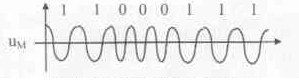
\includegraphics[scale=1.0]{8_fsk.png}
		\caption{Az FSK moduláció}
\end{figure}
A frekvencia moduláció (FSK) átlagértéke zérus, és ezért - szűrővel leválasztva - nem befolyásolja az aktuális ellenőrző jel ($Y_M$), illetve a végrehajtó jel ($u$) effektív értékét.
Megjegyzés: "D" generációs villamos a "C" generációs   helyére minden nehézség nélkül betehetők. (Természetesen fordítva nem lehetséges!) A belső áramköreik digitálisak. $D/A$ illetve $A/D$) átalakítókkal kifelé analóg működésűnek látszanak.$$$$
Az "E" generációs (Field busz-, azaz terepi busz) rendszerű távadók kimeneti, illetve végrehajtók bemeneti jele digitális távirat. Az "E" generációs eszközök használati értéke és "intelligenciája" azonos a "D" generációs távadókéval, de a kábelezési költségük lényegesen kisebb. Megjegyzés: Az "E" generációs, úgynevezett terepi buszos eszközök nem csereszabatosak a "C" és a "D" generációs eszközökkel!			
Jelenleg a legelterjedtebb típus a "C" generációs villamos távadó, végrehajtó. A generációs villamos távadók, illetve végrehajtók táplálásának négyféle változatát alkalmazzák.
\begin{figure}[hbtp]
    	 \centering
		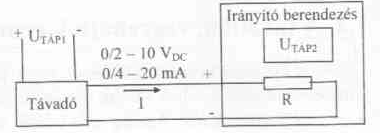
\includegraphics[scale=1.0]{9_negyvez_tav.png}
		\caption{A négyvezetékes távadók vezetékezése}
\end{figure}
$$$$
A négyvezetékes (9. ábra), ($24 V_{DC}$ vagy $230 V_{AC}$  tápellátású) távadó, és $24 V_{DC}$ tápellátású irányító berendezés.
\\\\
A négyvezetékes végrehajtó vezetékezése nagyon hasonlít a 9. ábráéhoz. Az analóg kimeneti modul áram-, vagy feszültséggenerátora szolgáltatja a végrehajtó felé a jelet. Az $R$ bemeneti ellenállás a végrehajtóban van. Értelemszerűen az áramnyíl iránya fordított.
\\\\
\begin{figure}[hbtp]
    	 \centering
		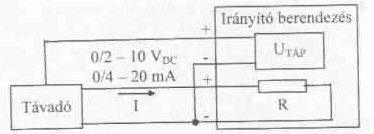
\includegraphics[scale=1.0]{10_haromvez_tav.png}
		\caption{A háromvezetékes távadók vezetékezése}
\end{figure}
A  háromvezetékes (10. ábra) távadó, és az irányító berendezés közös $24 V_{DC}$ tápellátású. A távadó és tápfeszültség földje a közös.
\\\\
\begin{figure}[hbtp]
    	 \centering
		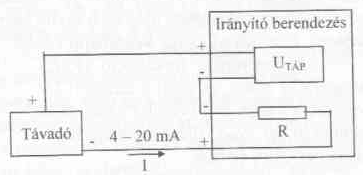
\includegraphics[scale=1.0]{11_ketvez_tav.png}
		\caption{A kétvezetékes távadók vezetékezése}
\end{figure}
A kétvezetékes ( 11.ábra) távadó, és az irányító berendezés, mint terhelés, sorban vannak kötve a közös $24 V_{DC}$ tápellátással.
A gyakorlati életben - a kábel költségek csökkentése miatt - a kétvezetékes távadókat alkalmazzák leggyakrabban, melyet az $IEC$ 1970-es
washingtoni ülésen elfogadott ajánlásban rögzítettek.
A háromvezetékes végrehajtó vezetékezése hasonlít a 10., a kétvezetékes végrehajtó vezetékezése pedig a 11. ábráéhoz.
$$$$
Szabványos ipari jeltartományok:
\begin{enumerate}
	\item[•]Analóg:\\
	Leggyakoribb $4-20 mA$, valamint $0-20 mA$\\
	Előfordul $0-10 V_{DC}$, $400-800 Hz$, $0.2-2 Bar$
	\item[•]Kétállapotú:\\
	Leggyakoribb $0-24 V_{DC}$\\
	($0-7 V$: Logikai nulla, $14-30 V$: Logikai 1)\\		Előfordul $0-230 V_{AC}$
	\item[•]Digitális:\\Ipari kommunikációs hálózatok
\end{enumerate}

\section{Ismertesse a vezérlés és a szabályozás közötti választás szempontját. Adja meg a jelátvivő tag fogalmát! A dimenzió nélkülivé tétel eljárása. A blokkdiagram átalakítás szabályai.}
\subsection{A vezérlés és a szabályozás közötti választás szempontja}
\subsubsection{Modell alkotás}
Az összetett irányítási feladatot fel kell bontani egyszerűbb, egymástól független feladatokra. Lehetőleg minden egyes irányított jellemző önálló feladat legyen!(Ez nem mindig lehetséges)
Mérésekkel (black box = fekete doboz modell), vagy az anyag és energia áramok egyensúlyi egyenleteit alkalmazva (grey box = szürke doboz modell) matematikai modellt kell készíteni az irányítási feladatokra.(A matematikai modell válasza a gerjesztő jelekre az előírt mérnöki pontossággal megegyezik fizikai rendszer viselkedésével.)
\subsubsection{Irányítási stratégia}
\begin{enumerate}
	\item[•]Vezérlés:\\
	Minden az irányított jellemzőre ható fizikai mennyiséget (jellemzőt) mérünk. Minden lehetséges körülmény esetén kielégítően pontos a modellünk. A beavatkozás a modell alapján történik.
	\item[•]Szabályozás: 
	Az irányított jellemzőt mérjük és a többi az irányított jellemzőre ható fizikai mennyiség eltérését az üzemi értéktől zavarnak tekintünk. Az irányított jellemzőt hasonlítjuk össze az előírt értékkel. A beavatkozás az eltérés megszüntetése érdekében történik. 
\end{enumerate}
\subsubsection{Stratégia választás}
Ha van kielégítő pontosságú modell, akkor alkalmazható a vezérlés.
Ha a szakasz modellezhető csupa kétállapotú jellel, akkor mindig alkalmazható vezérlés.\\Lehet analóg jellemző (nyomás, szint, stb.), ha a modellhez elég csak azt tudni, hogy egy értéknél kisebb vagy nagyobb.
Analóg jeleket tartalmazó irányítást vezérléssel megoldani általában költséges.\\Az analóg  mérés drágább, mint a kétállapotú, általában egynél több jellemzőt kell mérni, és idővel (kopás, öregedés, évszakok váltakozása, stb.) a rendszer modell paraméterei megváltoznak.
\subsubsection{Vezérlés kétállapotú jelekkel}
A Bool algebra szabályaival definiálható az algoritmus.
Az algoritmus zárt szekvenciákból épül fel.\\If…than   else, Do…until,  stb. A fejlesztő szoftverek gyakran felkínálnak grafikus megjelenítő felületeket, valamint kész, jól tesztelt szubrutinokat (funkció blokkok, függvények).
Berendezéscsoport, technológia irányításakor a feladatok nagyobb hányada On/Off vezérlés.Iparágtól függően az összes feladat $75-95\%$ On/Off vezérlés. A vész rendszer mindig, a védelmi rendszer szinte mindig csupa kétállapotú vezérlés. Az indítás, üzemeltetés, normál leállás folyamata tipikus sorrendi vezérlés.
\subsubsection{Szabályozás}
A SISO (Single Input Single Output) feedback (negatívan visszacsatolt) struktúra lefedi a szabályozási feladatok döntő hányadát.
Összetett (Cascade, Feedforward) szabályozások.Iparágtól függően a szabályozási feladatok $1-7\%$-a.
A MIMO (Multi Input Multi Output) és a adaptív (öntanuló) struktúra.Tipikus MIMO alkalmazás  a repülő gép vagy tankerhajó navigáció és a festő, hegesztő, stb. robot irányítás, illetve adaptív szabályozás a folyamatirányítás (Process Control) szabályozási feladatainak $1-2\%$-a.
\subsection{A jelátvivő tag fogalma}
Az irányítástechnika jelátvivő tagként vizsgál minden olyan alkatrészt (pl.: műveleti erősítő, szelep, stb.), szervet (pl.: jelillesztő áramkör, szivattyú, nyomás-, szint-távadó, stb.), illetve technológiai egységet (pl.: tartály, hőcserélő, autokláv, kazán, stb.), amelyeknek egy számunkra fontos jele, jellemzője (kimeneti jel, jellemző) jól befolyásolható egy számunkra könnyen változtatható jellemzőjével, jelével (bemeneti jel, jellemző). \\\\
Jelátvivő tagnak tekinthető minden technológia, berendezés, alkatrész, részegység, stb., amennyiben két jellemzője vagy jele között ok-okozati összefüggés állapítható meg. A jelátvivő tag be-, és kimeneti jele vagy jellemzője közötti összefüggés megadható egyenlettel vagy grafikusan. A be-, és a kimenet állandósult állapotai közötti összefüggés a statikus karakterisztika. A dinamikus viselkedés differenciál egyenlettel írható le az időtartományban  és átviteli függvénnyel a körfrekvencia vagy az operátoros tartományban.
\subsection{A dimenzió nélkülivé tétel eljárása.}
A valóságos fizikai rendszerekben a jellemzőknek van dimenziójuk. Az ipari méréstechnikában a villamos mennyiségeken (áram [$A$], feszültség [$V$], frekvencia
[$Hz$]) túl, a nagy ötöst (hőmérséklet [$^\circ C$], nyomás [$bar$], szint [$m$], áramlás [$\frac{kg}{sec}$] vagy
[$\frac{m^3}{sec}$], és a forgó mozgáshoz tartozó szögsebesség [$\frac{rad}{sec}$] vagy szögelfordulás [$rad$]) a leggyakrabban mért fizikai jellemző. De egyéb fizikai jellemző (pl.: $pH$ érték) is előfordulhat.
A jeltartományok is jelentősen különbözhetnek. Például teremhőmérséklet szabályozásakor $5 ^\circ C-35 ^\circ C$, hőkezelő kemence hőmérséklet szabályozásakor $200 ^\circ C-650 ^ \circ C$ között lehet az irányított jellemző értelmezési tartománya, vagy egy sávszűrő
működhet a [$MHz$] vagy a [$GHz$] tartományban.
Nagyban segíti az irányítási rendszerek egységes tárgyalását, ha a hatásvázlatban
(blokkdiagramban vagy jelfolyam ábrában) a jelek, jellemzők dimenzió nélküliek,
és azonos jelkészletűek.$$$$
Bármelyik jel, csak az időtől függő, {0 – 1} számtartománybeli számmá konvertálható:$$x\left(t\right)= \frac{x\left(t\right)\left[dim\right]-x_{min}\left[dim\right]}{x_{max}\left[dim\right]-x_{min}\left[dim\right]}$$
Az fenti kifejezéssel dimenzió nélkülivé tett jellemző értékekkel végzett számítások eredményét – ami egy számérték – értelmezni kell, vagyis az alábbi kifejezéssel ismét dimenziót kell rendelni hozzá.
$$x\left(t\right)\left[dim\right]=\left(x_{max}\left[dim\right]-x_{min}\left[dim\right]\right)*x\left(t\right)+x_{min}\left[dim\right]$$
A {0 – 1} számtartománybeli szám használata nem komfortos, ezért szokás az M (10, 100, esetleg egyéb) értékével beszorozni:
$$x\left(t\right)= \frac{x\left(t\right)\left[dim\right]-x_{min}\left[dim\right]}{x_{max}\left[dim\right]-x_{min}\left[dim\right]} * M$$
Megjegyzés: Az ipari irányítástechnikában az $M=100$ gyakran alkalmazott,
mert sokszor jobban értelmezhető, hogy a tartály $60\%$-ra van feltöltve, a szelep $45\%$-kosan nyitott, mint egy konkrét számérték. De természetesen az adott feladatnak megfelelően
célszerű "M" értékét megválasztani.
\subsection{A blokkdiagram átalakítás szabályai}
A blokkvázlat átalakítási szabályok felhasználásával (12-17. ábrák) átalakítható
a blokkvázlat, és így a soros, párhuzamos, visszacsatolt eredők számításának szabályai
már alkalmazhatók. Így egyszerűbb, könnyebben kezelhető formára hozható egy összetett blokkvázlat.
\begin{figure}[hbtp]
    	 \centering
		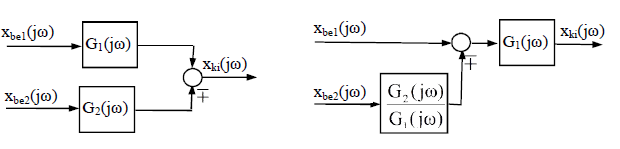
\includegraphics[scale=1.0]{12_osszegzo_blokk_ele.png}
		\caption{Összegző pont áthelyezése blokk elé}
\end{figure}
\begin{figure}[hbtp]
    	 \centering
		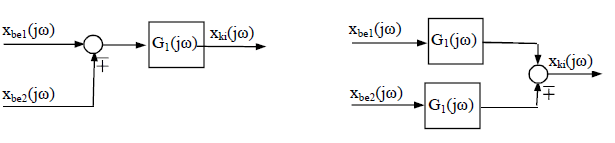
\includegraphics[scale=1.0]{13_osszegzo_blokk_moge.png}
		\caption{Összegző pont áthelyezése blokk mögé}
\end{figure}
\begin{figure}[hbtp]
    	 \centering
		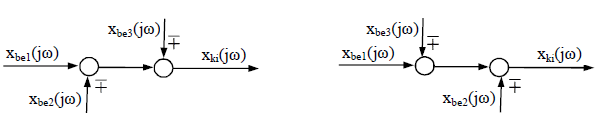
\includegraphics[scale=1.0]{14_osszegzo_blokk_megcserel.png}
		\caption{Összegző pont megcserélése}
\end{figure}
\begin{figure}[hbtp]
    	 \centering
		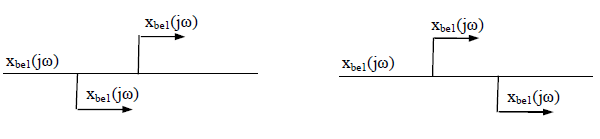
\includegraphics[scale=1.0]{15_elagazas_blokk_megcserel.png}
		\caption{Elágazási pont megcserélése}
\end{figure}
\begin{figure}[hbtp]
    	 \centering
		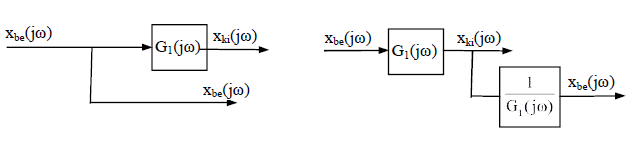
\includegraphics[scale=1.0]{16_elagazas_blokk_moge.png}
		\caption{Elágazási pont áthelyezése blokk mögé}
\end{figure}
\begin{figure}[hbtp]
    	 \centering
		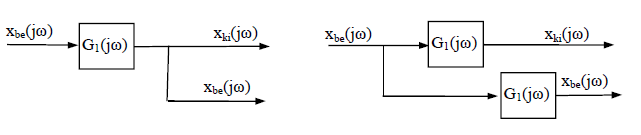
\includegraphics[scale=1.0]{17_elagazas_blokk_ele.png}
		\caption{Elágazási pont áthelyezése blokk elé}
\end{figure}
\newpage
\section{A vezérlés hatásvázlat. A vezérlési szekvencia fogalma. A kontaktusvezérlés szabályai. A funkció blokk és a függvény meghívása létra diagramban.}
\subsection{A vezérlés hatásvázlata}

\begin{figure}[hbtp]
    	 \centering
		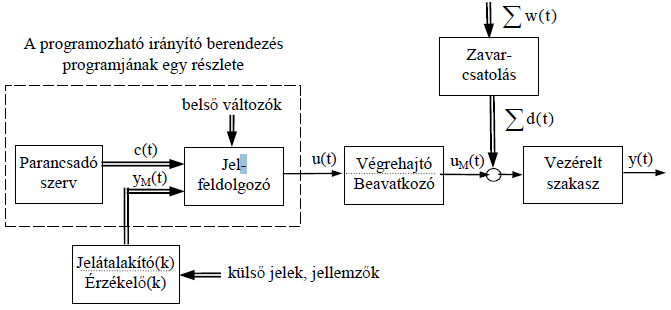
\includegraphics[scale=1.0]{18_vezerles_hatas.png}
		\caption{Vezérlés hatásvázlata}
\end{figure}
\subsection{A kontaktusvezérlés szabályai.}
Irányítástechnikai programozási nyelvek:
\begin{enumerate}
	\item Strukturált szöveg (ST: Structural Text)
	\item Funkciótérkép (FC: Function Chart)
	\item Utasítás soros (IL: Instruction Line)
	\item Létra diagram (LD: Ladder Diagram)
\end{enumerate}
Létra diagram:\\\\
Alacsony szintű, grafikus programozási nyelv. Szintaktikája a kontaktus
logikán alapul. A kontaktus logikában a kontaktusok és a tekercsek kétállapotú
változók. A kontaktusokon átfolyó áram gerjeszti a tekercset és a gerjesztett tekercs
meghúzza (a nyitottat zárja, a zártat nyitja) a hozzátartozó kontaktusokat.
Alaphelyzetben a nyitott kontaktus a ponált értéket és a zárt kontaktus negált
értéket jelent. Az MSz EN 61131-3 szerinti grafikus jelölések:
\begin{figure}[hbtp]
    	 \centering
		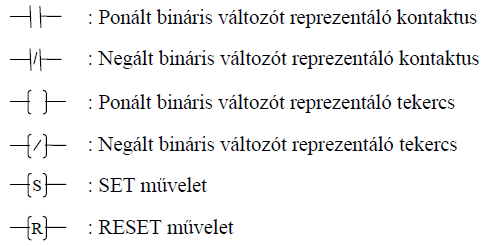
\includegraphics[scale=0.8]{19_letra_jeloles.png}
		\caption{}
\end{figure}
Programozáskor a változók szimbolikus neve a változók felett jelenik
meg. A sorba kötött kontaktusok AND kapcsolatba, a párhuzamosan kötött
kontaktusok OR kapcsolatban vannak. Kizáró vagy (EXOR) kapcsolat megvalósításához
a változót reprezentáló ponált és negált kontaktusra is szükség van.\\\\
A szubrutinhívás nem része az eredeti kontaktus
logikának. MSz EN 61131-3 LD programozási
nyelvben a szubrutinhívást egy téglalap jelképezi,
amelynek baloldalán a bemeneti változók, jobboldalán a kimeneti változók csatlakoznak. A téglalap felett van a típus, és afelett a szimbolikus név. A szubrutin memória területet foglal le a be és kimeneti változói részére, ami a szimbolikus név alapján címezhető (pl.: Időzítő.S).
A szubrutin bemeneti változóihoz hozzá kell
rendelni a feladat be- és kimeneti, vagy belső változóit.
A nem kétállapotú változókat széjjelhúzott kontaktus
jelképezi. A szubrutin kimeneti változóihoz
csak akkor kell tekercset hozzárendelni, ha
fizikai kimenethez akarjuk csatlakoztatni.\\\\
Funkcióblokk diagram (FBD: Function Block Diagram)
Alacsony szintű, grafikus programozási nyelv. Szintaktikája a digitális alapáramkör logikán alapul. A digitális alapáramkör logika több bemenetű
AND, OR, stb. logikai kapukkal írja le a megvalósítandó feladatot.
Az MSz EN 61131-3 FBD programozási
nyelvben a logikai műveleteket négyzet jelképezi,
amelynek baloldali hosszabbított éléhez a logikai
függvény argumentum változói, jobboldalához az eredményváltozó csatlakozik. A négyzetben van jelezve a logikai függvény típusa. A négyzetbe írt $\&$ az AND, a
"$\ge1$" az OR és a "=1" az EXOR logikai kapcsolatot
jelenti. A négyzet csatlakoztatási pontjainál elhelyezett
üres karika a változó negált értékét jelzi.
Az MSz EN 61131-3 FBD programozási
nyelvben a szubrutinhívást szintén egy téglalap jelképezi.
A szubrutin be és kimeneti változóihoz hozzá
kell rendelni a feladat be és kimeneti, vagy belső
változóit. Nem szükséges a szubrutin minden be és
kimeneti változójához értéket rendelni.
\\\\
A vezérlő relé programozás logikája,
hogy ha egy változó egy logikai
függvény argumentumában van, akkor
kontaktus, és ha a logikai függvény
eredménye, akkor tekercs szimbolizálja.
Tekercs lehet fizikai kimenet Q,
vagy belső M memória terület, valamint
szubrutinnal megvalósított grafikus objektum
(időzítő T és R, számláló C, D, és
R, szövegblokk TX, RX stb.) engedélyező,
törlő, vagy egyéb bemenete.
\\\\
Kontaktus lehet fizikai bemenet I, vagy belső M memória terület, valamint
szubrutinnal megvalósított grafikus objektum (időzítő T, számláló C, stb.)
kimeneti eredmény változója. Továbbá vannak szubrutinnal megvalósított speciális
kontaktusok (számláló komparátor V, analóg komparátor A, stb.).
Megjegyzés: Az időzítő, számláló, szövegblokk engedélyező tekercsének
lehelyezése jelenti a szubrutinhívást. Az időzítő, számláló stb., tekercseinek
vagy kontaktusának lehelyezési sorrendje tetszőleges. Ugyancsak szubrutinhívás
a számláló komparátor, analóg komparátor, stb. speciális kontaktusok
használata.
A kontaktusok alapállapota lehet "Normally open" záró (ponált változó)
és "Normally closed" bontó (negált változó). A lehelyezett kontaktust kijelölve,
a jobb egér klikk felhoz egy menü ablakot, amelyből a kívánt állapot kiválasztható.
\section{A szabályozási körnek milyen szabványos megnevezésű elemei és jelei vannak? Mi a munkaponti linearizáció, és hogyan dönthető el, hogy mekkora tartományra alkalmazható? A szabályozási kör egyensúlyi helyzetének beállítása a szabályozó jellegének megválasztásával.}
\subsection{A szabályozási körnek milyen szabványos megnevezésű elemei és jelei vannak?}
\begin{figure}[hbtp]
    	 \centering
		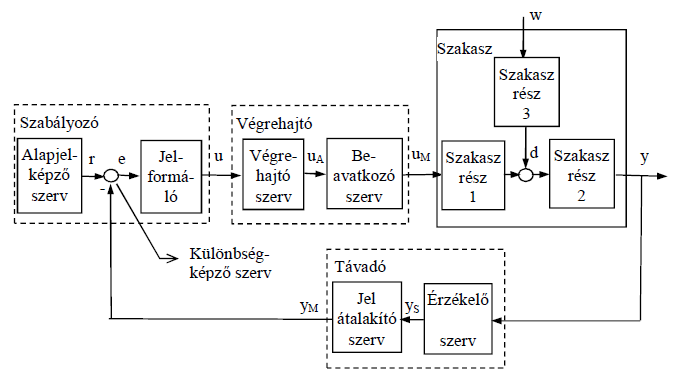
\includegraphics[scale=0.8]{20_szabalyozas_blokk.png}
		\caption{A szabályozási kör részletes blokkvázlata}
\end{figure}

Az szabályozási körökben a szakasz kivételével szervnek neveznek minden
irányítástechnikai funkcióval rendelkező eszközt. A 20. ábrán a szervek elnevezései a
blokkokba vannak beírva. A szaggatott vonallal körülhatárolt szervcsoportoknak önálló
nevük is van (szabályozó, végrehajtó, távadó) és gyakran egy jelátviteli tagként kezelik
ezeket, kivéve a szabályozó berendezést.
\\\\
A 20. ábrán látható szervek és berendezések feladata:
\begin{enumerate}
	\item[--] A szabályozó (controller) berendezés magába foglalja az alapjel-képző. különbségképző,
és a jelformáló szerveket.
	\begin{itemize}
		\item[•]Az alapjel-képző szerv (reference input element) feladata, hogy előállítsa az $Y_D$
alapértéknek megfelelő, az $Y_M$ ellenőrző jellel azonos értékkészletű és dimenziójú $R$ alapjelet.
\item[•]A különbségképző szerv (error detector) feladata, hogy összehasonlítsa az $R$
alapjel, és az $Y_M$ ellenőrző jel aktuális értékeit. A két jel különbsége az $e$ rendelkező
jel, amit gyakran hibajelnek is neveznek.
\item[•]A jelformáló (compensator) szerv feladata, hogy biztosítsa a visszacsatolt hurok
stabilitását, és az előírt minőségi paramétereit. A jelformáló szerv, és így a szabályozó
berendezés kimeneti jele az $U$ végreható jel. A jelformáló szervet gyakran kompenzáló tagnak nevezik.
	\end{itemize}
\end{enumerate}
Ha a szabályozó mikroprocesszor alapú, akkor a fenti szervek szoftver taszkok.
\begin{enumerate}
	\item[--] A végrehajtó (actuator) berendezés működteti a folyamatáramot (anyag vagy energia)
módosító a beavatkozó szervet. A beavatkozót működtető eszközt is végrehajtó
szernek nevezi a magyar szakirodalom.
	\begin{itemize}
		\item[•]A beavatkozó szerv (final element) feladata, hogy a szabályozott berendezés
vagy technológia működését befolyásoló $U_M$ módosító jellemzőt az $U_A$ beavatkozó
jelnek megfelelő értékre állítsa.
\item[•]A végrehajtó szerv (actuator drive) feladata, hogy működtesse a beavatkozó
szervet, és az $U$ végrehajtó jelnek megfelelő pozícióba állítsa. Ha a pontosság
érdekében visszaméri az $U_A$ beavatkozó jelet és összehasonlítja az előírt $U$ végrehajtó
jellel, akkor helyzetbe-állító szervnek nevezik.
	\end{itemize}
	\item[--]A szabályozott berendezés, technológia, szakasz (controlled equipment, process, plant)
előírt működése az irányítás célja.
\begin{itemize}
	\item[•]Ha a zavaró jellemző hatását is figyelembe kell venni, akkor – a blokkvázlat készítés
szabályának megfelelően - a jellemzéséhez két jelátviteli blokk, és egy
összegző szükséges.
\end{itemize}
\item[--]A távadó (transmitter) berendezés magába foglalja az $Y$ szabályozott jellemzőt
közvetlenül érzékelő szervet és a jelátalakítót.
\begin{itemize}
\item[•]Az érzékelő szerv (sensor) feladata, hogy az $y$ szabályozott jellemző értelmezési
tartományát minél pontosabban leképezze az $Y_S$ érzékelt jel értelmezési tartományába.
\item[•]A jelátalakító szerv (transducer) feladata, hogy nagyobb távolságra torzulás mentesen
továbbítható, és egyszerűen feldolgozható $Y_M$ ellenőrző jellé alakítsa az $Y_S$ érzékelt jelet.
\end{itemize}
\end{enumerate}
A szabályozási kör blokkvázlata megnevezés alatt leggyakrabban a 21. ábrán
látható elrendezést értik.
\begin{figure}[hbtp]
    	 \centering
		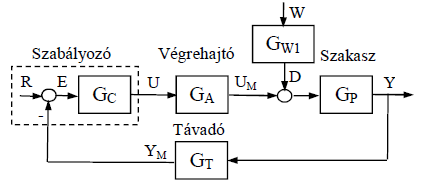
\includegraphics[scale=1.0]{21_szabalyozas_blokk_II.png}
		\caption{A szabályozási kör blokkvázlata}
\end{figure}
A 22. ábra az ipari berendezések szabályozásának azt a gyakori esetét reprezentálja,
amikor az irányító berendezés felöl nézve – az $u$ végrehajtó jel, mint bemenet,
és az $y_M$ ellenőrző jel, mint kimenet között – az irányított terület (process field) egyetlen
blokkal modellezett. Így a visszacsatoló ágban a jelátvitel 1. Ezt merev visszacsatolásnak
(unit feedback) nevezik.
\begin{figure}[hbtp]
    	 \centering
		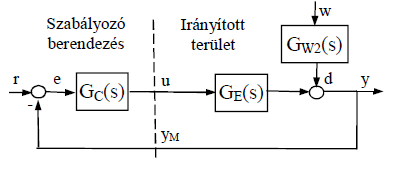
\includegraphics[scale=1.0]{22_szabalyozas_blokk_merev_vcs.png}
		\caption{A szabályozási kör merev visszacsatolású blokkvázlata}
\end{figure}
\\\\
A szabályozás célja, hogy az $Y$ szabályozott jellemző – a tranziensek lezajlása
után – előírt hibahatáron belül tartsa vagy kövesse az $R$ alapjel által előírt $Y_D$ alapértéket,
valamint előírt hibahatáron belülre csökkentse a $W$ zavaró jellemző üzemi értéktől
való eltérésének a hatását. Ehhez statikusan illeszteni kell a szabályozási kört, és dinamikusan
méretezni kell a kompenzáló tagot.
\subsection{Mi a munkaponti linearizáció, és hogyan dönthető el, hogy mekkora tartományra alkalmazható}
A jelátvivő tag lehet önbeálló, vagy lehet direkt vagy inverz jellege. Ha növekvő
bemenő jel értékekhez tartozó válaszjel állandósult állapotbeli értéke nő, akkor
a jelleg direkt, ha a válaszjel állandósult állapotbeli értéke csökken, akkor inverz. Az
önbeálló rendszereknek van statikus karakterisztikája. Az egyhurkos szabályozási kör
négy berendezése (20. ábra) közül legalább kettőnek önbeállónak kell lennie.
Megjegyzés: Leggyakrabban a szabályozó nem önbeálló. Gyakran a szakasz, és
ritkán a végrehajtó. A távadó mindig önbeálló, hisz a szabályozott jellemzőt kell leképeznie.
A 24. ábrán csak a szabályozó nem önbeálló.
\begin{figure}[hbtp]
    	 \centering
		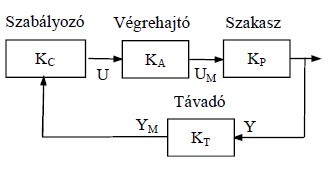
\includegraphics[scale=1.0]{23_szabalyozas_stat.png}
		\caption{A szabályozási kör statikus blokkvázlata}
\end{figure}
Megjegyzés: A 23. ábrán a szabályozó
berendezés – eltérően a 21. ábrától – egy blokként
van ábrázolva és a zavaró jellemző hatását
a 24. ábrán vesszük figyelembe.
\begin{figure}[hbtp]
    	 \centering
		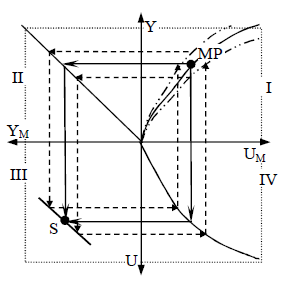
\includegraphics[scale=1.0]{24_szabalyozas_karak.png}
		\caption{A statikus karakterisztikák illesztése}
\end{figure}

Megjegyzés: A 23. ábrán a G(s) átviteli függvények helyett a berendezések statikus
karakterisztikáinak a vizsgált munkaponthoz tartozó átviteli tényezői vannak a
berendezések blokkjaiba írva. Ez a vizsgálatban nem játszik szerepet.
\\\\
A 24. ábra egy olyan speciális koordináta rendszer, amelynek minden
síknegyedében a 23. ábra berendezéseinek be-, és kimenete van, a 23. ábra nyílirányainak
megfelelően egymáshoz képest $+90^\circ$-al el vannak forgatva. A négy koordináta rendszer origója közös.
\\\\
A 24. ábra "I" jobb felső síknegyedében a szakasz $Y=F\left(U_M\right)$ statikus (állandósult
állapotbeli) karakterisztikája van. A folytonos vonal az átlagos zavar jellemző értékek
mellett meghatározott statikus karakterisztika. A szaggatott pont-vonalak a zavar
jellemzők hatását, más szavakkal az Y szabályozott jellemző állandósult értékei változásának
határait mutatja.
\\\\
A 24. ábra "II" bal felső síknegyedében a távadó $Y_M =F\left(Y\right)$ statikus karakterisztikája
van. A karakterisztika nem szükségszerűen, de szerencsére sokszor lineáris a
teljes jeltartományban. A 24. ábrán a távadó statikus karakterisztikája lineáris.
A 24. ábra "IV" jobb alsó síknegyedében a végrehajtó $UM =F\left(U\right)$ statikus karakterisztikája
van. Számos irányítástechnikai előnnyel bír, ha a végrehajtó statikus karakterisztikája lineáris. Sajnos legtöbbször, így a 24. ábrán is, a végrehajtó statikus karakterisztikája nem lineáris.
\\\\
A statikus jel illesztés fontos szabálya, hogy a jelek, jellemzők végértékei illeszkedjenek
egymáshoz. A 24. ábrán ez teljesül, a pontozott vonal keretezi a jelek,
jellemzők végértékeit (a kezdeti értékek az origóban vannak).
Megjegyzés: Ez a műszerező mérnök feladata. Olyan távadót választani, ami
képes a szabályozott jellemző teljes jeltartományát mérni. Olyan végrehajtót választani,
amely képes elegendően nagy módosító jellemzőt szolgáltatni.
A szabályozott szakasz kívánatos "MP" munkapontját a technológus definiálja,
és ez mindig berajzolható az I. síknegyedbe. A 24. ábrán a szakasz statikus karakterisztikájú,
és így az "MP" munkapontja az üzemi statikus karakterisztika görbéjén van.
Ha a zavaró jellemző eltér a tervezett üzemi értékétől, akkor a statikus karakterisztika
is módosul (az ábrán szaggatott vonal, dupla pont görbék). A munkapontból balra vetítve
a távadó munkapontja, lefelé vetítve a végrehajtó munkapontja jelölhető ki a távadó,
illetve a végrehajtó statikus karakterisztikáin (hegyes, folytonos nyilak).
\\\\
A 24. ábra "III" bal alsó síknegyedében a szabályozó van. A mérnöki gyakorlatban
fontos eldönteni, hogy a szabályozó jellege direkt vagy inverz legyen. A távadó
munkapontjából lefelé és a végrehajtó munkapontjából balra vetítve (hegyes, folytonos
nyilak) a 24. ábra "III" bal alsó síknegyedében kijelölhető az "S" pont.
Az "S" ponton átfektetett direkt vagy inverz meredekségű egyenessel dönthető
el, hogy melyik szabályozó jelleget kell alkalmazni az adott szabályozási körben. A
24. ábrán az inverz jelleg (növekvő $Y_M$ ellenőrző jel értékéhez az $U$ végrehajtó jel
csökkenő értéke tartozik) bizonyult megfelelőnek. Más statikus jelleggörbék esetén lehet
a direkt jelleg a megfelelő választás!
Inverz jellegű statikus karakterisztikájú szabályozó esetén, ha zavar hatására
hirtelen megnő vagy lecsökken az $Y$ szabályozott jellemző értéke, akkor a szaggatott
nyilak mentén végighaladva az eredeti $Y$ szabályozott jellemző értékének közelébe térünk
vissza a 24. ábrán.\\\\
Megjegyzés: A maradó szabályozási eltérést a kompenzáló tag dinamikai viselkedése
szüntetheti meg.\\\\
Könnyű ellenőrizni, hogy ha a szabályozási kör statikus karakterisztikái a 24.
ábra szerintiek, akkor direkt meredekségű egyenest átfektetve az "S" ponton az $Y$ szabályozott
jellemző értéke távolodik az eredeti "MP" munkapontbeli értékétől.
Megjegyzés: Ha a szabályozó jellegét rosszul választják meg, akkor semmilyen
kompenzáló algoritmus nem tudja megakadályozni, hogy a szabályozott jellemző ne
valamelyik végértékére üljön ki.\\\\
Ha a szakasz nem önbeálló jellegű, akkor a 24. ábra "I" jobb felső
síknegyedében, a tervezett "MP" munkapontban – a szabályozó berendezéshez hasonlóan
– kell a szakasz direkt vagy inverz jellegének megfelelő direkt vagy inverz
meredekségű vetítő egyenest berajzolni. Ezután a szabályozó statikus jellegének megkeresése
ugyanúgy történik, mint az önbeálló szakasznál.
\section{A mintavételi idő megválasztása szürke doboz modell esetén.  Mi a helyzet domináns időállandóval rendelkező eredő szakasz esetén? A mintavételi idő megválasztása fekete doboz modell esetén az átmeneti függvényből, valamint a körfrekvencia függvényből. Mi a helyzet az integráló jellegű eredő szakasz esetén?}
A hibrid szabályozásokat tervezés szempontjából analóg szabályozásként szokás
kezelni. Ennek feltétele a $T_S$ mintavételi idő helyes megválasztásával a felharmonikus összetevőkből származó hiba néhány ezreléknél kisebb legyen.
Szürke doboz modell esetén ismertek az eredő szakasz időállandói. Fekete doboz
modell esetén az eredő szakasznak vagy az időtartánybeli átmeneti függvénye
vagy a körfrekvencia tartománybeli átviteli függvény grafikus megjelenítése (Bode diagram) lett méréssel meghatározva.
\subsection{Szürke doboz modell alapján}
Ha ismert az eredő szakasz átviteli függvénye, akkor ismertek a pólusai is. A
pólusok abszolút értékek reciprok értéke az eredő szakasz $T_k$ időállandói. Ha a $T_S$ mintavételi
idő megválasztásakor eleget teszünk az alábbi ajánlásnak, akkor a mintavételezésből
származó hiba legfeljebb néhány ezrelék.
$$\frac{\sum_{k=1}^{K}{T_k}}{50} \geq T_S \geq \frac{\sum_{k=1}^{K}{T_k}}{150}$$ahol $K$ a pólusok száma.
Ha az eredő szakasz közel $PT1$ jellegű vagy rendelkezik egy domináns időállandóval, akkor nagyobb számmal {100-150} célszerű osztani, hiszen az amplitúdó viszonylag magas körfrekvenciákon sem csökken meredeken.
Ha az eredő szakasz három vagy több időállandóval rendelkezik és nincs köztük
domináns, akkor kisebb számmal {50-100} célszerű osztani, hiszen az amplitúdó
meredeken csökken a nagyobb körfrekvenciákon.
Ha integráló jellegű az eredő szakasz, akkor az eredő szakasz Bode alakjának
időállandóit (köztük a TI integrálási időt) kell összegezni.
\subsection{Szürke doboz modell, átmeneti függvény alapján}
Nagyjából az időállandók összegének ötszöröse a $2\%$-
os és négyszerese az $5\%$-os pontosságú beállási idő. Az előbbi kifejezés alapján:$$\frac{T_{a2\%}}{250} \geq \frac{T_{a2\%}}{750}$$
$$\frac{T_{a5\%}}{200} \geq \frac{T_{a5\%}}{600}$$
Az átmeneti függvény alakjából kell következtetni időállandók számára és közelségére.
Ezt követően az osztó paraméter megválasztásának szempontjai azonosak.
Integráló jellegű eredő szakasz esetén az $IT1$ szakaszközelítésnek megfelelő $T_I$
integrálási időnek és $T_g$ látszólagos időállandónak az összegét kell osztani legalább
{500-750} közötti számmal. Minél távolabb vannak egymástól, annál nagyobbal.\\
Megjegyzés: A szürke és fekete doboz modell esetén is igaz, hogy ha valóságos
holdidő van az eredő szakaszban, akkor a holtidő legyen egész számú többszöröse a
mintavételi időnek.
\subsection{Szürke doboz modell, körfrekvencia átviteli függvény alapján}
Az algoritmus feldolgozásának idő igénye $T_S$ időtartamú jelkésleltetést – $H$
holtidős tagot - hoz a szabályozási körbe, ami torzítja a $G_0\left(j\omega\right)$ felnyitott hurok átviteli
függvény fázismenetet. A holtidős tag fázisa lineárisan csökken, vagyis aránypárba állítható
a körfrekvencia és a hozzátartozó fázistolás.\\
Megjegyzés: A Bode diagramon a logaritmikus lépték miatt csökken exponenciálisan
a holtidős tag fázisa.\\
Ha a holtidős tag fázismenetén a $2\omega_{s}$ körfrekvencián engedünk $1\left[rad\right]$ fázistolást és az $\omega_C$ vágási körfrekvencián a holtidős tag fázistolása $\Delta \phi$, akkor érvényes az
alábbi kifejezés. A kifejezésben az $\omega_{s}$ a mintavételi körfrekvencia.
$$\frac{\Delta \phi\left[rad\right]}{1\left[rad\right]} = \frac{\omega_C \left[\frac{rad}{sec}\right]}{2\omega_S \left[\frac{rad}{sec}\right]}$$
a körfrekvencia diagramon számértékre $\omega_S = \frac{1}{T_S}$\\
Ha nincs vágási körfrekvencia, akkor a legkisebb törésponti körfrekvenciát kell
a fenti kifejezésben felhasználni.
Ha az eredő szakasz leendő vágási körfrekvenciáján csak néhány fokos fázistorzulást {0.015-0.075$\left[rad\right]$} eredményezhet a mintavétel, akkor:
$$0.015\left[rad\right]\leq \frac{\omega_C * T_S}{2}\left[rad\right]\leq0.075\left[rad\right]$$
$$\frac{0.03}{\omega_C}\left[sec\right] \leq T_S \left[sec\right] \leq \frac{0.15}{\omega_C} \left[sec\right]$$
Az eredő szakasz körfrekvencia függvényének fázismenetén jól látható az időállandók
száma, és amplitúdó menetén az időállandók egymáshoz való közelsége. A
konstans {0.03-0.15} megválasztásának megfontolása azonos az előzőekével.
Szokás a vágási körfrekvencián megengedett fázistorzulás mértékével definiálni
a mintavételi időt. A $\Delta \phi$ dimenzióját fokra váltva:
$$\frac{\pi \left[rad\right]}{\Delta \phi \left[\circ\right]}$$
Szakasz modell közelítés esetén a közelítő időállandók az ismertek. Mindig 100 feletti értékkel osszuk az időállandók összegét! Integráló jellegű szakasz esetén a válaszfüggvény egyenletesen növekvő (csökkenő) részének amplitúdó változása haladja meg a bemeneti jel állandósult amplitúdó változásának mértékét! 
\section{A jelátviteli alaptagok átviteli függvényei, átmeneti függvényei, differenciál egyenletei, Bode diagramjaik.}
\subsection{P (proportional) arányos tag}
Differenciálegyenlet:$$x_{ki}\left(t\right) = K * x_{be}\left(t\right)$$
Körfrekvencia átviteli függvény:$$G\left(j\omega\right) = K$$
A decibel érték átszámítása: $$K = 10^\frac{K\left[dB\right]}{20}$$
\begin{figure}[hbtp]
    	 \centering
		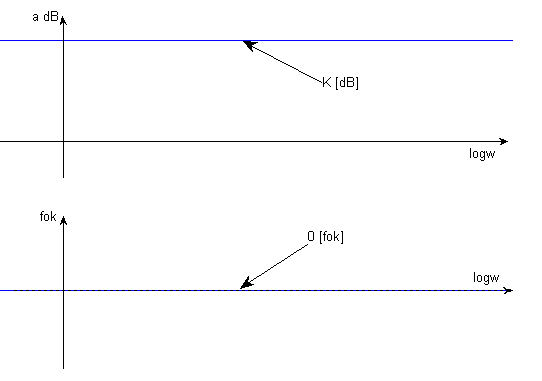
\includegraphics[scale=1.0]{25_p_tag_bode.png}
		\caption{Az arányos alaptag Bode diagramja}
\end{figure}
\begin{figure}[hbtp]
    	 \centering
		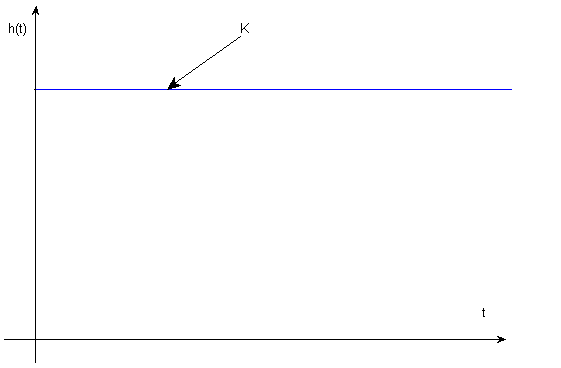
\includegraphics[scale=1.0]{26_p_tag_atmenet.png}
		\caption{Az arányos alaptag h(t) átmeneti függvénye}
\end{figure}
\newpage
\subsection{I (integral) integráló tag}
Differenciálegyenlet:$$x_{ki}\left(t\right) = K_I \int_0^\infty x_{be}\left(t\right)dt$$
$$T_I\frac{dx_{ki}\left(t\right)}{dt} = x_{be}\left(t\right)$$
Körfrekvencia átviteli függvény:$$G\left(j\omega\right) = \frac{K_I}{j\omega} = \frac{1}{j\omega T_I} = \frac{1}{j\frac{\omega}{\omega_I}}$$
\begin{figure}[hbtp]
    	 \centering
		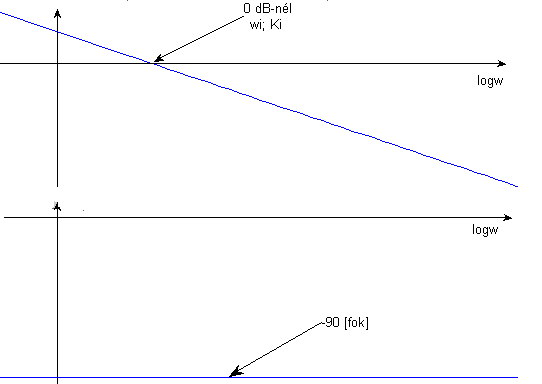
\includegraphics[scale=1.0]{27_i_tag_bode.png}
		\caption{Az integráló alaptag Bode diagramja}
\end{figure}
\begin{figure}[hbtp]
    	 \centering
		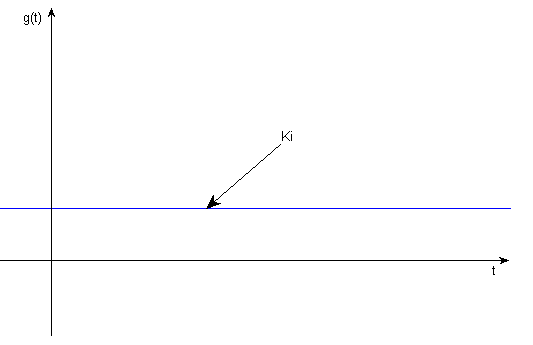
\includegraphics[scale=1.0]{28_i_tag_atmenet.png}
		\caption{Az integráló alaptag g(t) súlyfüggvénye és h(t) átmeneti függvénye}
\end{figure}
\newpage
\subsection{D (derivative) differenciáló tag}
Differenciálegyenlet:$$x_{ki}\left(t\right) = K_D\frac{dx_{be}\left(t\right)}{dt}$$
$$x_{ki}\left(t\right) = T_D\frac{dx_{be}\left(t\right)}{dt}$$
Körfrekvencia átviteli függvény:$$G\left(j\omega\right) = K_D j\omega = j\omega T_D = j\frac{\omega}{\omega_D}$$
\begin{figure}[hbtp]
    	 \centering
		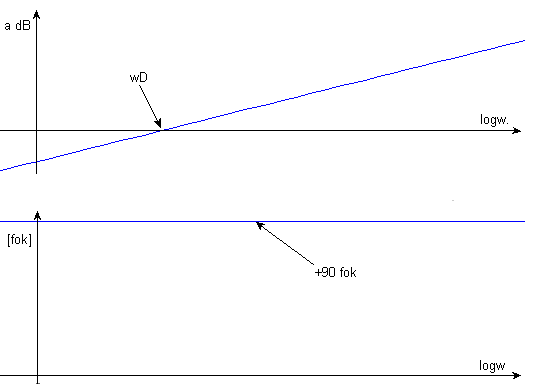
\includegraphics[scale=1.0]{29_d_tag_bode.png}
		\caption{Differenciáló alaptag Bode diagramja}
\end{figure}
\newpage
\subsection{H holtidős (dead time, transport time, delay time) tag}
Differenciálegyenlet:$$x_{ki}\left(t\right) = K * 1\left(t-\tau\right)x_{be}\left(t-\tau\right)$$
Körfrekvencia átviteli függvény:$$G\left(j\omega\right) = e^{j\omega\tau}$$
\begin{figure}[hbtp]
    	 \centering
		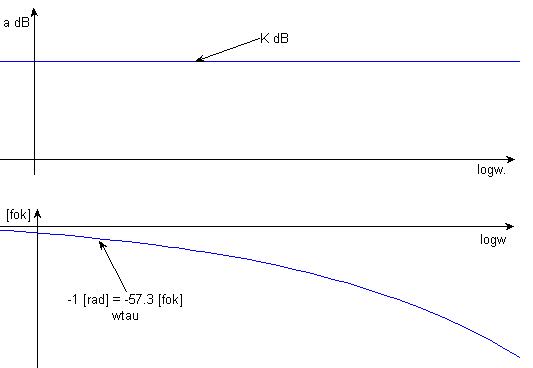
\includegraphics[scale=1.0]{30_ht1_tag_bode.png}
		\caption{Holtidős alaptag Bode diagramja}
\end{figure}
\begin{figure}[hbtp]
    	 \centering
		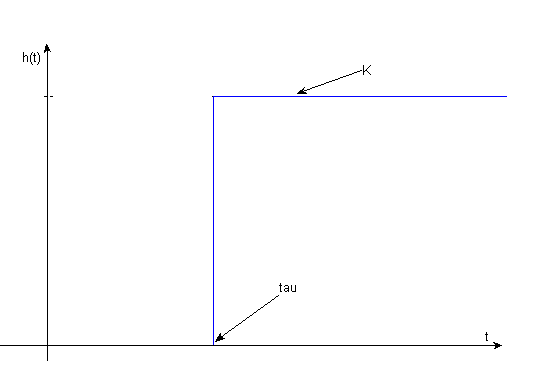
\includegraphics[scale=1.0]{31_ht1_tag_atmenet.png}
		\caption{Holtidős alaptag átmeneti függvénye}
\end{figure}
\newpage
\subsection{PT1 egy időállandós (first order) tag}
Differenciálegyenlet:$$T\frac{dx_{ki}\left(t\right)}{dt} + x_{ki}\left(t\right) = K * x_{be}\left(t\right)$$
Körfrekvencia átviteli függvény:$$G\left(j\omega\right) = \frac{K}{j\omega * T + 1}=\frac{K}{j\frac{\omega}{\omega_T} + 1}$$
\begin{figure}[hbtp]
    	 \centering
		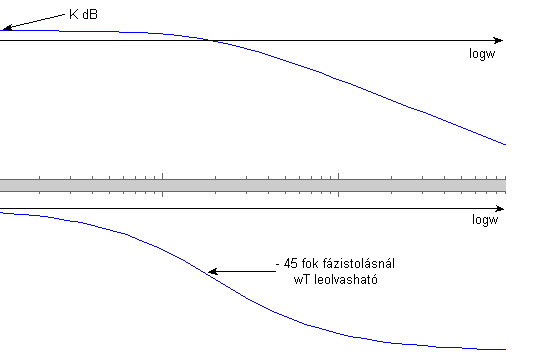
\includegraphics[scale=1.0]{32_pt1_tag_bode.png}
		\caption{Egy tárolós alaptag Bode diagramja}
\end{figure}
\begin{figure}[hbtp]
    	 \centering
		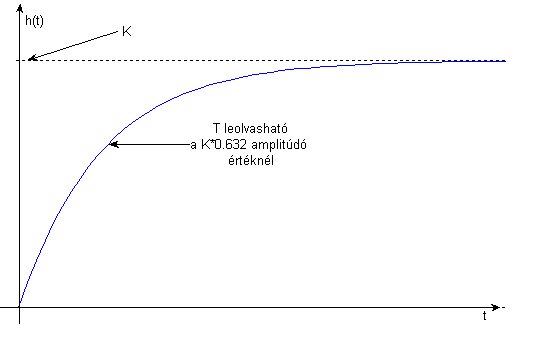
\includegraphics[scale=1.0]{33_pt1_tag_atmenet.png}
		\caption{Egy tárolós alaptag átmeneti függvénye}
\end{figure}
\newpage
\subsection{PT2 két időállandós (second order) tag}
Differenciálegyenlet:$$T^2 \frac{d^2 x_{ki}\left(t\right)}{dt^2} + 2 * D * T\frac{dx_{ki}\left(t\right)}{dt} + x_{ki}\left(t\right) = K * x_{be}\left(t\right)$$
Körfrekvencia átviteli függvény:$$G\left(j\omega\right) = \frac{K}{T^2\left(j\omega\right)^2 + 2 * D * T * j\omega + 1}$$
\begin{figure}[hbtp]
    	 \centering
		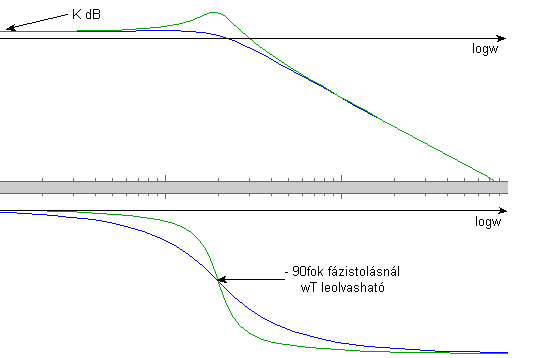
\includegraphics[scale=1.0]{34_pt2_tag_bode.png}
		\caption{Két tárolós alaptag Bode diagramja}
\end{figure}
\begin{figure}[hbtp]
    	 \centering
		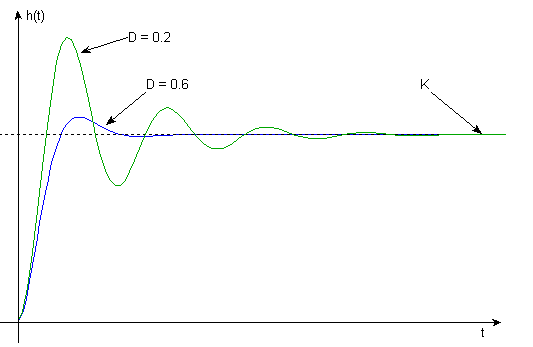
\includegraphics[scale=1.0]{35_pt2_tag_atmenet.png}
		\caption{Két tárolós alaptag átmeneti függvénye}
\end{figure}
\newpage
\section{Az átviteli függvények soros, párhuzamos, visszacsatolt eredője.}
\subsection{Soros eredő}
$$x_1\left(j\omega\right) = G_1\left(j\omega\right) * x_{be}\left(j\omega\right)$$
$$x_{ki}\left(j\omega\right) = G_2\left(j\omega\right) * x_1\left(j\omega\right)$$
Behelyettesítéssel megkapható a soros eredő:
$$G_{12}\left(j\omega\right) = G_1\left(j\omega\right) * G_2\left(j\omega\right)$$
\begin{figure}[hbtp]
    	 \centering
		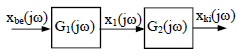
\includegraphics[scale=1.0]{36_soros.png}
		\caption{Soros kapcsolás}
\end{figure}
\subsection{Párhuzamos eredő}
$$x_1\left(j\omega\right) = G_1\left(j\omega\right) * x_{be}\left(j\omega\right)$$
$$x_2\left(j\omega\right) = G_2\left(j\omega\right) * x_{be}\left(j\omega\right)$$
Összegzéssel a párhuzamos eredő:
$$G_{12}\left(j\omega\right) = G_1\left(j\omega\right) \mp G_2\left(j\omega\right)$$
\begin{figure}[hbtp]
    	 \centering
		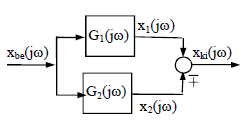
\includegraphics[scale=1.0]{37_parhuzamos.png}
		\caption{Párhuzamos kapcsolás}
\end{figure}
\subsection{Visszacsatolt eredő}
$$x_1\left(j\omega\right) = x_{be}\left(j\omega\right) \mp x_2\left(j\omega\right)$$
$$x_{ki}\left(j\omega\right) = G_1\left(j\omega\right) * x_1\left(j\omega\right)$$
$$x_2\left(j\omega\right) = G_2\left(j\omega\right) * x_{ki}\left(j\omega\right)$$
Az $x_1\left(j\omega\right)$ és az $x_1\left(j\omega\right)$ segédváltozókat kiejtve kapjuk a $$x_{ki}\left(j\omega\right) = G_1\left(j\omega\right)\left[x_{be}\left(j\omega\right) \mp G_2\left(j\omega\right) * x_{ki}\left(j\omega\right) \right]$$ kifejezést, majd ezt a kifejezést rendezve, a visszacsatolt eredő:
$$G_{12}\left(j\omega\right) = \frac{G_1\left(j\omega\right)}{1 \pm G_1\left(j\omega\right) G_2\left(j\omega\right)}$$
\begin{figure}[hbtp]
    	 \centering
		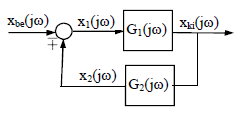
\includegraphics[scale=1.0]{38_visszacsatolt.png}
		\caption{Visszacsatolt kapcsolás}
\end{figure}
\section{A zárt szabályozási kör átviteli függvényei. A HPT1, IT1, PT3 tag átmeneti függvénye és átviteli függvénye. Az átmeneti függvényen hol olvashatók le a paraméterek?}
\subsection{A zárt szabályozási kör átviteli függvényei}
\subsubsection{Felnyitott hurok átviteli függvény}
$$G_0\left(s\right) = \frac{y_M\left(s\right)}{r\left(s\right)} = G_C\left(s\right)G_A\left(s\right)G_P\left(s\right)G_T\left(s\right)$$
\subsubsection{Alapjel átviteli függvény}
$$G_{yr}\left(s\right) = \frac{y\left(s\right)}{r\left(s\right)} = \frac{G_C\left(s\right)G_A\left(s\right)G_P\left(s\right)}{1+G_C\left(s\right)G_A\left(s\right)G_P\left(s\right)G_T\left(s\right)} ;w = 0$$
\subsubsection{Hibajel átviteli függvény}
$$G_{er}\left(s\right) = \frac{e\left(s\right)}{r\left(s\right)} = \frac{1}{1+G_C\left(s\right)G_A\left(s\right)G_P\left(s\right)G_T\left(s\right)}; w = 0$$
\subsubsection{Zavar átviteli függvény}
$$G_{yw}\left(s\right) = \frac{y\left(s\right)}{w\left(s\right)} = \frac{G_{W1}\left(s\right)G_P\left(s\right)}{1+G_C\left(s\right)G_A\left(s\right)G_P\left(s\right)G_T\left(s\right)}; r = 0$$
\subsubsection{Zavar, hibajel átviteli függvény}
$$G_{ew}\left(s\right) = \frac{e\left(s\right)}{w\left(s\right)} = \frac{-G_{W1}\left(s\right)G_P\left(s\right)G_T\left(s\right)}{1+G_C\left(s\right)G_A\left(s\right)G_P\left(s\right)G_T\left(s\right)}; r = 0$$
\subsection{IT1 tag átmeneti függvénye, paraméterei}
$$G_{IT1}\left(s\right) = \frac{1}{sT_I}\frac{1}{sT+1}$$
$$T_I = \frac{t_3 - t_2}{a\left(t_3\right)- a\left(t_2\right)}$$
$$T = t_1$$
\begin{figure}[hbtp]
    	 \centering
		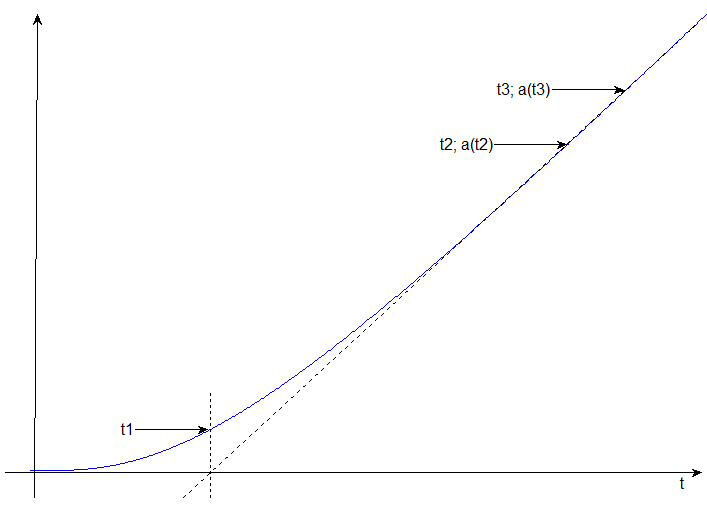
\includegraphics[scale=0.5]{39_it1_atmeneti.png}
		\caption{Az eredő szakasz átmeneti függvénye}
\end{figure}
\begin{figure}[hbtp]
    	 \centering
		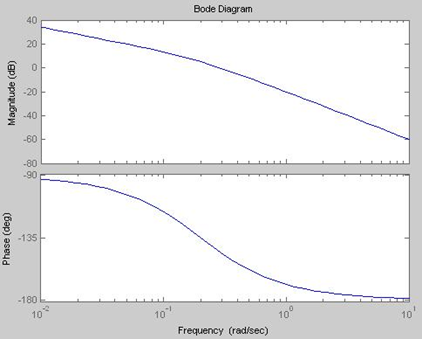
\includegraphics[scale=1.0]{40_it1_bode.png}
		\caption{Az eredő szakasz Bode diagramja}
\end{figure}
\\\\
\subsection{HPT1 tag átmeneti függvénye, paraméterei}
$$G_{HPT1}\left(s\right)=K_P\frac{1}{sT + 1}e^{-s\tau}$$
\begin{figure}[hbtp]
    	 \centering
		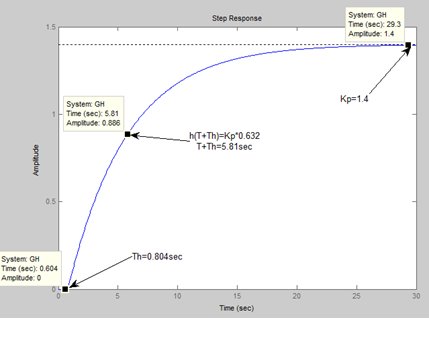
\includegraphics[scale=0.8]{41_hpt1_atmeneti.png}
		\caption{Az eredő szakasz átmeneti függvénye}
\end{figure}
\begin{figure}[hbtp]
    	 \centering
		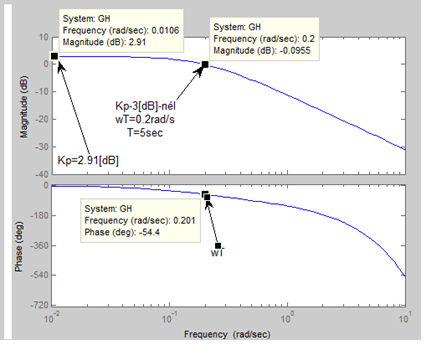
\includegraphics[scale=0.8]{42_hpt1_bode.png}
		\caption{Az eredő szakasz Bode diagramja}
\end{figure}
\subsection{PT3 tag átmeneti függvénye, paraméterei}
$$G_{PT3}\left(s\right)=\frac{K_P}{\left(sT_1+1\right)\left(sT_2+1\right)\left(sT_3+1\right)}$$
\begin{figure}[hbtp]
    	 \centering
		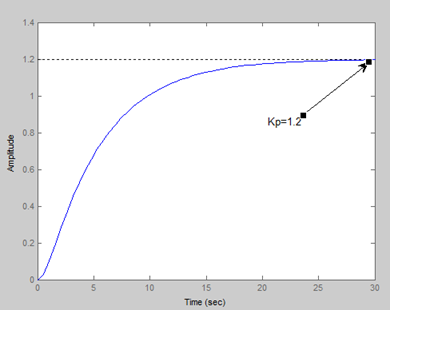
\includegraphics[scale=0.8]{43_pt3_atmeneti.png}
		\caption{PT3 tag átmeneti függvénye}
\end{figure}
\begin{figure}[hbtp]
    	 \centering
		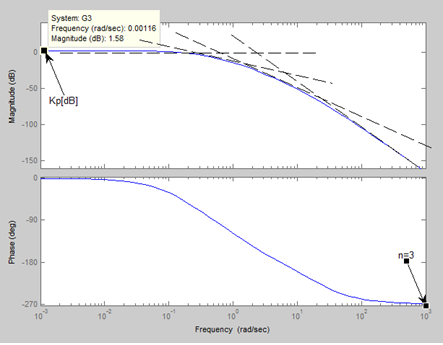
\includegraphics[scale=0.8]{44_pt3_bode.png}
		\caption{PT3 tag Bode diagramja}
\end{figure}
\section{Adja meg az PIDT kompenzáló tag felépítését és a lehetséges átviteli függvényeit! A lehetséges átviteli függvények közül melyik milyen szakasz esetén előnyös?}
\section{Adja meg az PI kompenzáló tag átviteli függvényét, Bode diagramját, valamint a leendő vágási körfrekvencia leolvasási pontját!}
\section{Adja meg az PDT kompenzáló tag átviteli függvényét, Bode diagramját, valamint a leendő vágási körfrekvencia leolvasási pontját!}
\section{Mi a szabályozási kör értékkövetése? Mitől függ értékkövetés esetén a maradó szabályozási eltérés? Melyik átviteli függvényből határozná meg a konkrét értékét?}
\section{Mi a szabályozási kör értéktartása? Mitől függ értéktartás esetén a maradó szabályozási eltérés? Melyik átviteli függvényből határozná meg a konkrét értékét?}
\section{Az átviteli függvény polinom tört, gyöktényezős, és Bode alakja. Mi a típusszám és melyik függvényből olvasható le? Mi a kapcsolat az átviteli függvény gyökei és időállandói között? }
\section{Minőségi jellemzők az időtartományban.}
\section{Stabilitás vizsgálat a zárt szabályozási kör átviteli függvényének gyökei alapján. Hogyan lehet a szabályozási kör gyökeiből az időtartománybeli minőségi jellemzőket megbecsülni? }
\section{Stabilitás vizsgálat a felnyitott hurokátviteli függvény alapján.}
\section{Milyen szakaszmodell közelítéseket ismer az arányos és integráló szakaszok azonosítására? Hogyan használhatók a közelítő modell paraméterei kompenzáláskor?}
\section{Mi a pólus kiejtéssel történő kompenzálás elve?}
\section{A fázistartalék és az erősítéstartalék fogalma. Hogyan választ kompenzáló tagot az eredő szakasz körfrekvencia függvényének (Bode diagramjának) ismeretében?}
\section{Hogyan határozza meg az eredő szakasz körfrekvencia függvényén a leendő vágási körfrekvencia értékét?}
\section{A PI kompenzálás menete a körfrekvencia tartományban. }
\section{A PDT kompenzálás menete a körfrekvencia tartományban. }

\tableofcontents
\end{document}